\chapter{Methods}
\label{cha:Methods}

\section{Task Description}

In this section describes the task and the simulation environment, which are the foundation of this thesis and will remain unchanged throughout the course of the project.
The task is to develop an agent using reinforcement learning that is able to complete a parcour in a simulated environment without collisions. The agent has to traverse the parcour by passing through a number of goals indicated by pairs of either red or blue blocks without collisions. This problem belongs to the class of single player continuous state and action space problems. The observation space of the agent consists of an image that is taken from its front facing camera. At each timestep the agent uses a neural network to process the image and produce two actions. The two actions are the acceleration values of the left and right wheel, being applied to the wheels until a new action is selected.
The task and agent are simulated using the Unity engine \ref{fig:unity}. The engine handles the rendering of the environment, collisions, agent movement and reward functions.
% The timesteps do not have a fixed duration, a new timestep is started as soon as the last one is finished. The amount of timesteps per minute will be measured? This is like FPS?

\begin{figure}
     \centering
     \subfigure[Example image of the agent at the start of a parcour with 3 goals in Unity]{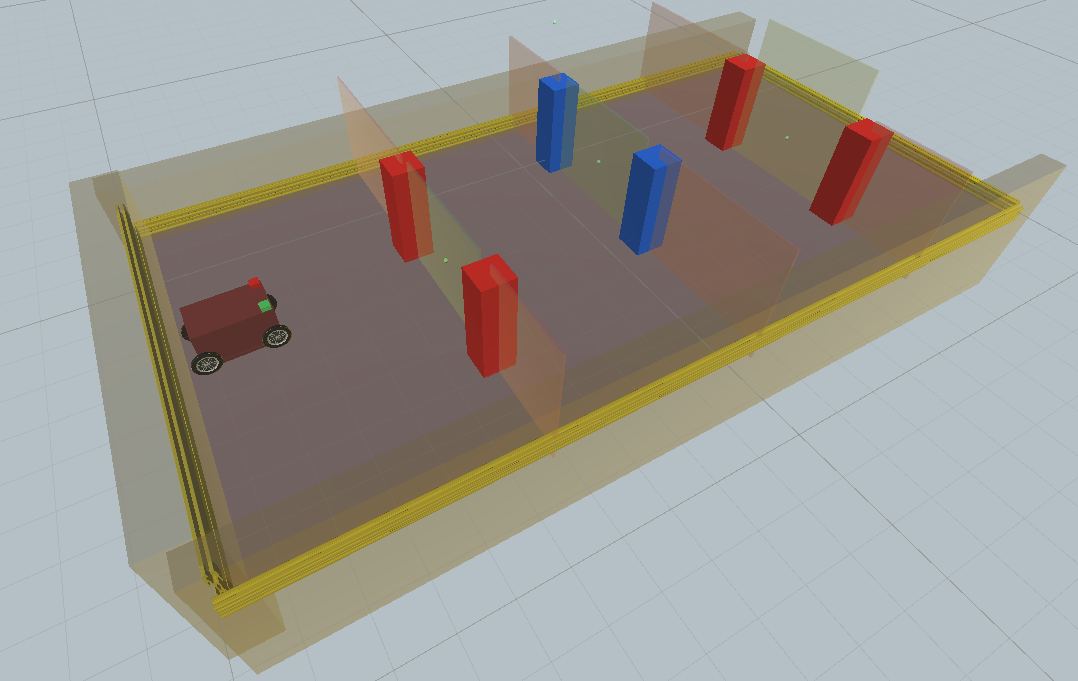
\includegraphics[width=0.4\textwidth]{Bilder/parcour.png}}\qquad
     \subfigure[Agent camera view]{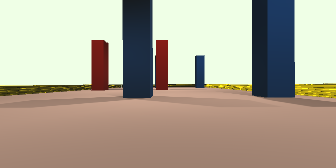
\includegraphics[width=0.4\textwidth]{Bilder/agent_image_from_unity.png}}\\
     \caption{Unity simulation environment and agent camera view}
     \label{fig:unity}
\end{figure}

% mention the similarity/simplicity of the task


\section{Reinforcement Learning Algorithm and Frameworks}

As outlined in the related works section, many different RL algorithms can be used to solve single player continuous state and action space problems. The PPO algorithm is most commonly used for problems of this class and has already been successfully used in the investigated task \autocite{maximilian}. The PPO algorithm will be used as discussed in Related Work.

In this thesis, the PPO algorithm from the stable-baselines3 library \autocite{sb3} will be used. The library is based on the PyTorch framework and provides APIs for training, logging, visualization and evaluating reinforcement learning agents. The training and evaluation algorithms can be modified easily. RL algorithms from stable-baselines3 are applied on Gymnasium environments \autocite{gymnasium}. As mentioned before the Unity simulation is integrated in a Gymnasium environment. The communication between Unity and the Gymnasium environment is realized using the Peaceful Pie library \autocite{peacefulpie}. The PyTorch framework is used to implement the convolutional neural network, see \ref{fig:unitycommunication} for a summary of the Unity-Python interaction.

\begin{figure}
     \centering
     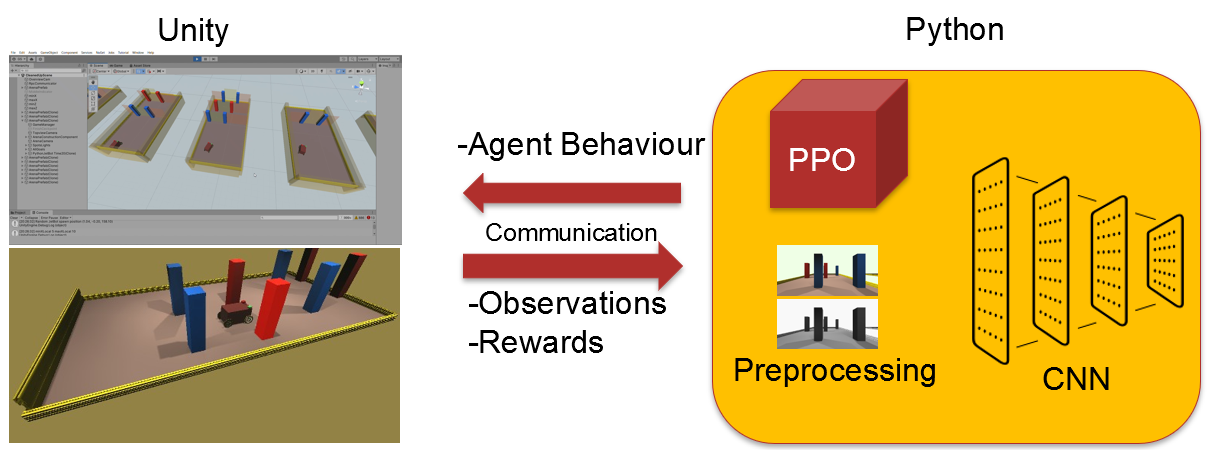
\includegraphics[width=0.8\textwidth]{Bilder/unity_communication.png}
     \caption{Unity and Python communication}
     \label{fig:unitycommunication}
\end{figure}

% maybe mention the similarity/simplicity of the task here to show PPO is good

\section{Reinforcement Learning Algorithm Details}

\subsection{Reward Function}
% drl_for_ad says reward shaping is good

The design of the reward function is crucial for the success of any reinforcement learning algorithm and agent. The reward function should encourage the desired behaviour. In our case, the agent should drive through all goals without collisions as quickly as possible. The previous work by \autocite{maximilian} awarded a reward of 100 for completing the parcours, a reward of 1 for passing a goal and a reward of -1 for missing a goal, colliding with a wall/obstacle and timeouts. This should encourage the agent to navigate the simulation without collisions and to pass through all goals, see EventReward \ref{fig:reward_function}. Furthermore a reward proportional to the agent's velocity at each step was awarded to encourage speed, resulting quick parcour completions, see VelocityReward \ref{fig:reward_function}.

The combination of the EventReward and VelocityReward includes everything needed to encourage the desired agent behaviour. However the agents might fail to learn to navigate the parcour, since the EventReward is very sparse. Reward shaping is the practise of providing reinforcement learning agents with frequent and accurate rewards. This helps the agent develop the desired behaviour quicker and more reliably since reward signals are less sparse and less delayed \autocite{drl_for_ad}. The VelocityReward can be considered as reward shaping since it provides the agent with a reward at each timestep.

Here the reward function will be further extended with a DistanceReward and OrientationReward, see \ref{fig:reward_function}. The DistanceReward is proportional to the difference in distance between the agent and the next goal during a timestep, this should encourage the agent to drive towards the next goal. The OrientationReward is proportional to the cosine similarity between the agent's direction and the direction towards the next goal, this should encourage the agent to drive in the direction of the next goal. The partial rewards are combined using a weighted sum. The weights will be determined during the experimentation phase. Setting a weight to zero will disable the corresponding reward shaping component.


\begin{figure}
     \centering
     \begin{align}
          R(s_t,a_t) &= c_1 \cdot DistanceReward(s_t,a_t) + c_2 \cdot OrientationReward(s_t,a_t) \nonumber \\
          &  + c_3 \cdot VelocityReward(s_t, a_t) + c_4 \cdot EventReward(s_t, a_t) \nonumber \\
          DistanceReward(s_t,a_t) &= \Delta distance(Agent, NextGoalPosition) \cdot \Delta T \nonumber \\
          OrientationReward(s_t,a_t) &= S_C(NextGoalPosition - AgentPosition, agentDirection) \cdot \Delta T \nonumber \\
          VelocityReward(s_t, a_t) &= v \cdot \Delta T \nonumber \\
          EventReward(s_t, a_t) &= \begin{cases}
               100,           \text{completed the parcour}           \\
               1,             \text{passed a goal}                   \\
               -1,            \text{missed a goal}                   \\
               -1,            \text{collision with wall or obstacle} \\
               -1,            \text{timeout}                         \\
               0,             \text{otherwise}                       \\
          \end{cases} \nonumber
     \end{align}
     \caption{Complete reward function R with all its components}
     \begin{tabular}{r@{: }l r@{: }l}
     $S_C$ & cosine similarity & $c_i$ & weights\\
     $s_t$& state t & $a_t$& action in state t 
     \end{tabular}
     \label{fig:reward_function}
\end{figure}
% cosine similarity is one for same direction, zero for orthogonal directions and -1 for opposite directions

\iffalse
\begin{figure}
     \[SmoothedReward(s_t,a_t) = \sum_{i=0}^{n} \gamma^{i} \cdot Reward(s_{t+i}, a_{t+i}) \]
     \caption{Reward Function that uses the reward of current timestep $t$ and the next $n-1$ timesteps, $\gamma$ is the discount factor (between 0 and 1)}
\end{figure}

% post: https://stackoverflow.com/questions/77626064/name-of-reward-function-that-utilizes-the-reward-of-the-next-n-steps
% https://ai.stackexchange.com/


Mein Ansatz zu n-step bootstrapping macht wenig Sinn, da die RL algorithmen bereits diese Art von Future Reward lernen
Siehe AI Stackexchange Frage https://ai.stackexchange.com/questions/43068/what-is-the-name-of-the-reward-function-that-utilizes-the-rewards-of-the-next-n

Es könnte Sinn machen zu beschreiben, wie das Environment diskretisiert wird und die Reward funktion mit dieser diskretisierten Step Funktion interagiert

\subsubsection{Dealing with delayed Rewards}
Delayed rewards can be a big problem in reinforcement learning and make the training process difficult. Delayed rewards are rewards that are not obtained immediately after the responsible action is taken. In our environment an action \(a_n\) (e.g. turning right) may lead to a collision at state \(s_{n+x}\) which results in a negative reward for action \(a_{n+x}\). The RL algorithm might fail learn to avoid the action \(a_n\).

There are a multiple approaches to dealing with delayed rewards. These approaches use the reward at the current timestep and the near future. These approaches result in a more accurate and dense reward signal and can improve the training stability and performance of the agent.
N-step bootstrapping uses the rewards at the current step and the next \(n\) steps \autocite{nstepbootstrapping}.
A similar approach does not use the reward from the next \(n\) steps but rather the cumulative reward encountered in the next \(n\) seconds \autocite{trackmania}. Due to the continuous nature of the environment this approach might be more suitable than N-step bootstrapping.

% TODO the algorithm in nstepbootstrapping is different from my implementation, check if it is correct
% the nstepbootstrapping in rlbook2020 describes the update targets of the neural network and requires value estimates from (one of) the next n steps
\begin{figure}
     \[BootstrappedReward(s_t,a_t) = R(s_t,a_t) + \gamma R(s_{t+1},a_{t+1}) + \gamma^2 R(s_{t+2},a_{t+2}) + ... + \gamma^n R(s_{t+n},a_{t+n})\]
     % TODO check if this bootstrapping corresponds to the one in the paper
     \caption{N-step bootstrapping reward function \autocite{nstepbootstrapping}}
\end{figure}
\fi


\subsection{Frame Stacking}

Two configurations of the agent by \autocite{maximilian} used a memory to enhance the agent's input. The memory consisted of the input from the last few steps of the agent. This technique of stacking the history has been widely used in RL for continuous \autocite{atari} and discrete action spaces \autocite{alphago}. This allows the agent to perceive object movement, time and velocities \autocite{atari}.
This frame stacking will also be used to enhance the agent's input, since the next goal may leave the agent's current field of vision.

% TODO image of frame stacking?

% However since the investigated environment does not have fixed timesteps this approach might not be as effective. The time elapsed between two steps can vary due to many factors such as varying compute resources. It could prove useful to provide the model with the input of the last few steps and in addition the elapsed time between these steps. % these few sentences only make sense if the varying time is dicussed in the first part of the Methods section

% test other memory mechanisms?
% like for example also feeding the previous time step's hidden layer activation as input
% that way the agent would know the previous "decision" not just the previous input
% not enough time, just use the same memory mechanism as in the previous work
% the memory question is not a goal anymore


\section{Implementation Details for Light Setting Robustness} \label{light_setting_robustness}

\subsection{Convolutional Neural Networks}

The works by \autocite{merlin_flach} and \autocite{maximilian} showed that the agent's performance greatly depended on the quality of the input preprocessing pipeline. This object detection pipeline had difficulties detecting objects under varying light settings. This thesis uses convolutional neural networks instead of a hand crafted object detection pipeline. CNNs with an adapted training process should make the agent more robust to varying light settings and improve the performance of the agent.
Convolutional networks are common practise in the field of reinforcement learning, due to the ability of these networks to adapt and process images. The convolutional neural network could potentially learn to identify relevant information in images more reliably than the previously used image detection pipeline. The research by \autocite{merlin_flach} showed that not all the information provided by the object detection pipeline was considered to be relevant by the neural network.
As a starting point for experimentation, the CNN architecture will be the same as \autocite{human_level_control}, which proved successful for simple control tasks.

% we use the default CnnPolicy network, is it the same as the one described in Atari?
% architecture: https://github.com/DLR-RM/stable-baselines3/blob/d671402c9373391f44d8a2ad11deed615e0f4bae/stable_baselines3/common/torch_layers.py#L89-L106
% it is exactly as described in "Human-level control through deep reinforcement learning"
% \autocite{atari} has a slightly smaller NN

% (more robustness?) (previous input was shit (sim2real paper wegen x, y, width, height input problem)) (previous system higly depended on bounding box detection)


\subsection{Feature Reduction and Preprocessing}

Several preprocessing approaches can be used to prepare an image, before processing it with convolutional neural networks. Downsampling, greyscaling and rescaling steps will be applied to the images. The goal of downsampling and greyscaling is to reduce the input space size. Both were used in the foundational Atari paper \autocite{atari}. This results in increased processing speed and can reduce the chance of overfitting of the network. The greyscaled images in \ref{fig:4bildchen} show that the colour information is not crucial, as the closest blocks remain easily recognizable. Reducing the input space size also helps the PPO algorithm, since more data entries fit in memory, which allows for more efficient training. Pixel values are rescaled to between 0 and 1, which can help the neural network learn quicker \autocite{jason}.

\subsection{Histogram Equalization}

The previous work this thesis builds upon used the HSV colour space to extract the differently coloured objects. Colours in this space consist of three values, referring to hue, saturation and brightness. The hue value was used for extracting the blue and red goal posts. In theory, the utilization of this colour space should make the object detection resilient to changes in brightness, since this information does not affect the hue value. However, this proved to be invalid in practice as shown by \autocite{maximilian}.
Convolutional neural network typically use the RGB colour space or a greyscale colour space. Image transformations such as brightness and contrast changes can be applied to images before they are processed by the CNN. A histogram equalization of the input images could play a big role in making the agent more resilient to changes in illumination. Image d) in \ref{fig:4bildchen} shows the effect of histogram equalization on an image, however the image looks worse for identifying the goal posts since the shadows became much darker. This suggests the equalization might not be necessary, nor useful. Therefore equalization and other preprocessing steps will be investigated during the implementation and experimentation phase.


%* histogram equalization / enhance contrast (preprocessing) https://stackoverflow.com/questions/39308030/how-do-i-increase-the-contrast-of-an-image-in-python-opencv

% \autocite*{drl_for_ad} shows a lot of best practises in RL for autonomous driving

\begin{figure}
     \centering
     \subfigure[Original Image]{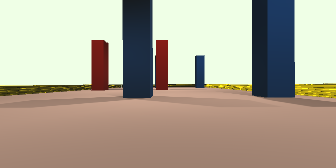
\includegraphics[width=0.5\textwidth]{Bilder/agent_image_from_unity.png}}\qquad
     \subfigure[Downsampled image]{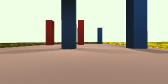
\includegraphics[width=0.25\textwidth]{Bilder/agent_downsampled.png}}
     \subfigure[greyscale]{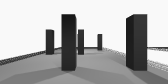
\includegraphics[width=0.25\textwidth]{Bilder/agent_grey.png}}\qquad
     \subfigure[histogram equalized image]{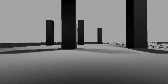
\includegraphics[width=0.25\textwidth]{Bilder/agent_equalized.png}}
     \caption{4 Stages of preprocessing images for the CNN}
     \label{fig:4bildchen}
\end{figure}


\section{Training Process}

\subsection*{Training Parcours}
The achieve good results, the PPO Reinforcement Learning algorithm requires the agent to be placed in a training environment similar to the evaluation environment \autocite{rlbook2020}. In the training process by \autocite{maximilian}, the goal objects were spawned semi-randomly with a minimum and maximum distance to the next goal. Two different training regimes were used. In Single-Goal-Training the episodes were stopped after completing the first goal or upon collision. In Full-Map-Training the episodes were stopped after completing the whole map or upon collision. The reasoning behind Single-Goal-Training is that the agent will encounter a bigger variety of states during training, since it will start at different positions in the parcour. However, the Full-Map-Training is closer to the evaluation scenario, since the agent has to complete multiple goals in succession during evaluation.
Single-Goal-Training performed worse than Full-Map-Training in the previous work \autocite{maximilian} for all evaluation parcours except for the difficult one.

These two approaches will be experimented with, in addition to another approach called Fixed-Training. The most successful approach will then be used for the remainder of the thesis. In Fixed-Training the agent will be trained on the same parcours that are later used for the evaluation. This is standard practise in the domain of Reinforcement Learning \autocite{rlbook2020}. In Fixed-Training, a random evaluation parcour is chosen to train the agent on in each episode.

\begin{figure}
     \centering
     \subfigure[Single-Goal-Training]{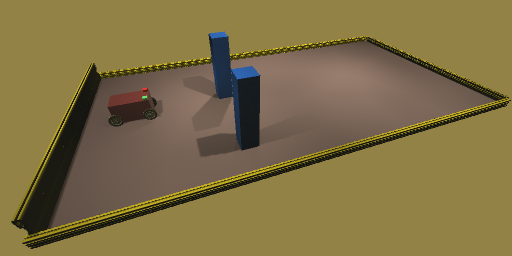
\includegraphics[width=0.3\textwidth]{Bilder/training_regime_sgt.png}}
     \subfigure[Full-Map-Training]{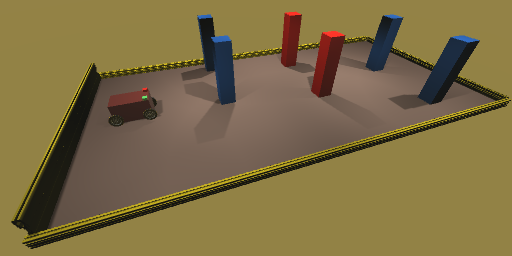
\includegraphics[width=0.3\textwidth]{Bilder/training_regime_fmt.png}}
     \subfigure[Fixed-Training (hard parcour)]{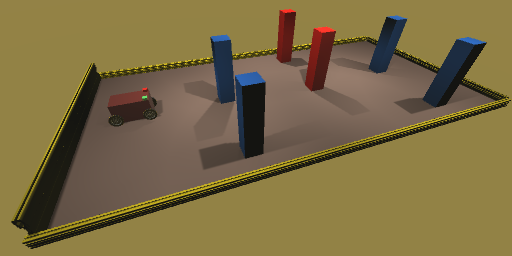
\includegraphics[width=0.3\textwidth]{Bilder/training_regime_fixed_hard.png}}
     \caption{Training regimes} 
     \label{fig:training_regimes}
\end{figure}


\subsection*{Training Light Settings}
Since the agent utilizes a Convolutional Neural Network to be resilient towards changing light conditions. Furthermore it is necessary to train the agent with varying light conditions, otherwise the adaptability of the CNN would not be fully utilized. This way, the agent will be able to generalize and learn to deal with different light conditions. The light conditions will be randomized for each training parcour similar to the light conditions during evaluation.
Training with fixed light settings could also provide interesting insight when comparing the results against training with varying light settings. This comparison would show if the varying light settings during training help in generalizing to different light settings.

% TODO light_setting_pov_reduced_lighting_no_preprocessing from image printer shows that the colours are not clear in reduced lighting, this justifies the use of greyscaling

% TODO do we need an image equalization if the network is trained on varying light conditions?
% Image printer needs to show this

\subsection*{Data Augmentation}

Convolutional Neural Networks require huge amounts of data to learn and generalize. Data augmentation is a technique to increase the amount training data by applying transformations to the collected data such as rotation, translation, scaling, flipping and colour changes. Data augmentation is inexpensive, since the new data points are not collected in simulation, as well as providing a more diverse set of training data. \autocite{conditional_imitation_learning_for_driving} employed a diverse set of data augmentation for their imitation learning approach to end-to-end-driving that used a CNN.

During the training process, the collected images will be augmented by applying random transformations to them. The transformations change the image similarly to how different environment conditions (e.g. lighting, camera quality and fog) might change the image. It is not yet decided which transformations will be used, possible candidates are changes in contrast, brightness and tone, as well as filters like Gaussian blur, Gaussian noise, salt-and-pepper noise.
Geometric transformations such as translations and rotations are not used since our control commands are not invariant to these transformations.

\begin{figure}
     \centering
     \subfigure[Original image]{
\includegraphics[width=0.3\textwidth]{Bilder/data_entry_original.png}}
     \subfigure[Gaussian Noise $\mu=0$ $\sigma=5$]{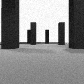
\includegraphics[width=0.3\textwidth]{Bilder/data_entry_augmented_gaussian_sigma_5.png}}
     \subfigure[salt-and-pepper noise]{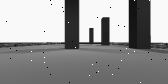
\includegraphics[width=0.3\textwidth]{Bilder/data_entry_augmented_salt_and_pepper.png}}
     \caption{Data augmentation examples}
     \label{fig:data_augmentation}
\end{figure}

% TODO find another paper with data augmentaton



% TODO wenn ", this" oder ", the" oder ", they" vorkommt ist es meist ein Run-on sentence, man sollte die Sätze aufteilen
% entweder mit einem Punkt oder mit einem Komma und einem Konjunktion (and, but, or, so, yet, which, therefore)